\section{Resolución Analítica}
Se ha dividido la resolución en diversas secciones:

\subsection{Análisis bajo incertidumbre}
En este primer análisis, no se conoce la probabilidad de cada estado de la naturaleza, por lo que la toma de decisiones se hace bajo criterios inciertos.

\subsubsection{Criterio de Laplace}
Bajo este criterio, se asume que los estados de la naturaleza son equiprobable, o de igual probabilidad, para construir un análisis simple de valores esperados. Bajo esta idea, tenemos:

\insertaligned[\label{eqn:laplace}]{
    \text{Valor esperado Decisión 1: } & 8 \cdot 0.5 + 7 \cdot 0.5 = 7.5    \\
    \text{Valor esperado Decisión 2: } & 14 \cdot 0.5 + 5 \cdot 0.5 = 9.5   \\
    \text{Valor esperado Decisión 3: } & 20 \cdot 0.5 - 9 \cdot 0.5 = 5.5
}

Bajo esto, nuestra mejor decisión es montar el edificio mediano.

\subsubsection{Criterio optimista}
También conocido como el criterio Maximax, consiste en utilizar el valor más alto de la tabla para guiar la decisión. El método es obtener el valor máximo de cada decisión para cada estado de la naturaleza, y elegir la decisión con el valor máxima de estas. Se presenta una nueva tabla con los valores más altos resaltados, con el valor más alto de estos mismos, en rojo:

\begin{table}[H]
    \begin{tabular}{r|cc|}
        \cline{2-3}
        \multicolumn{1}{l|}{}                                   & \multicolumn{2}{l|}{\textbf{Estado de la naturaleza}}                                       \\ \hline
        \multicolumn{1}{|l|}{\textbf{Alternativas de Decisión}} & \multicolumn{1}{l|}{Alta Demanda}                       & \multicolumn{1}{l|}{Baja Demanda} \\ \hline
        \multicolumn{1}{|r|}{Edif. Pequeño}                     & \multicolumn{1}{c|}{\textbf{8}}                         & 7                                 \\
        \multicolumn{1}{|r|}{Edif. Mediano}                     & \multicolumn{1}{c|}{\textbf{14}}                        & 5                                 \\
        \multicolumn{1}{|r|}{Edif. Grande}                      & \multicolumn{1}{c|}{{\color[HTML]{CB0000} \textbf{20}}} & -9                                \\ \hline
    \end{tabular}
\end{table}

Bajo este criterio optimista, es de nuestro interés seleccionar el edificio grande, pues es el que tiene el más alto beneficio potencial.

\subsubsection{Criterio pesimista}
Este criterio ligeramente antagónico al anterior consta de una estrategia similar, sin embargo, donde la idea era obtener el valor más alto potencial, en este criterio buscamos el valor más bajo de la peor situación. En otras palabras, obtenemos el valor mínimo de cada decisión para cada estado de la naturaleza, y seleccionamos el valor máximo entre cada decisión. Debido a esto, este criterio recibe el nombre de Minimax.

En la siguiente tabla, similar a la anterior, se presenta en negrita los valores más bajos para cada decisión, y con un color rojo el valor seleccionado.

\begin{table}[H]
    \begin{tabular}{r|cc|}
        \cline{2-3}
        \multicolumn{1}{l|}{}                                   & \multicolumn{2}{l|}{\textbf{Estado de la naturaleza}}                                     \\ \hline
        \multicolumn{1}{|l|}{\textbf{Alternativas de Decisión}} & \multicolumn{1}{l|}{Alta Demanda}                     & \multicolumn{1}{l|}{Baja Demanda} \\ \hline
        \multicolumn{1}{|r|}{Edif. Pequeño}                     & \multicolumn{1}{c|}{8}                                & {\color[HTML]{FE0000} \textbf{7}} \\
        \multicolumn{1}{|r|}{Edif. Mediano}                     & \multicolumn{1}{c|}{14}                               & \textbf{5}                        \\
        \multicolumn{1}{|r|}{Edif. Grande}                      & \multicolumn{1}{c|}{{\color[HTML]{333333} 20}}        & \textbf{-9}                       \\ \hline
    \end{tabular}
\end{table}

Bajo este criterio pesimista, es de nuestro interés seleccionar el edificio pequeño, pues es el que incurre en el beneficio más alto en su peor situación

\subsubsection{Matriz de arrepentimiento}
Este criterio consta en buscar la decisión donde se pierda menos beneficio entre la mejor y peor decisión. Para esto, se genera una nueva tabla, donde se resta el valor más alto de cada decisión por el valor de la decisión en el estado de la naturaleza a evaluar. En términos prácticos, se obtiene lo siguiente:

\begin{table}[H]
    \begin{tabular}{r|cc|}
        \cline{2-3}
        \multicolumn{1}{l|}{}                                   & \multicolumn{2}{l|}{\textbf{Estado de la naturaleza}}                                     \\ \hline
        \multicolumn{1}{|l|}{\textbf{Alternativas de Decisión}} & \multicolumn{1}{l|}{Alta Demanda}                     & \multicolumn{1}{l|}{Baja Demanda} \\ \hline
        \multicolumn{1}{|r|}{Edif. Pequeño}                     & \multicolumn{1}{c|}{8 - 8}                            & {\color[HTML]{333333} 8 - 7}      \\
        \multicolumn{1}{|r|}{Edif. Mediano}                     & \multicolumn{1}{c|}{14 - 14}                          & 14 - 5                            \\
        \multicolumn{1}{|r|}{Edif. Grande}                      & \multicolumn{1}{c|}{{\color[HTML]{333333} 20 - 20}}   & 20 - (-9)                         \\ \hline
    \end{tabular}
\end{table}

La tabla final, que llamaremos matriz de arrepentimiento, se ve de la siguiente manera:

\begin{table}[H]
    \begin{tabular}{r|cc|}
        \cline{2-3}
        \multicolumn{1}{l|}{}                                   & \multicolumn{2}{l|}{\textbf{Estado de la naturaleza}}                                     \\ \hline
        \multicolumn{1}{|l|}{\textbf{Alternativas de Decisión}} & \multicolumn{1}{l|}{Alta Demanda}                     & \multicolumn{1}{l|}{Baja Demanda} \\ \hline
        \multicolumn{1}{|r|}{Edif. Pequeño}                     & \multicolumn{1}{c|}{0}                                & {\color[HTML]{333333} 1}          \\
        \multicolumn{1}{|r|}{Edif. Mediano}                     & \multicolumn{1}{c|}{0}                                & 9                                 \\
        \multicolumn{1}{|r|}{Edif. Grande}                      & \multicolumn{1}{c|}{{\color[HTML]{333333} 0}}         & 29                                \\ \hline
    \end{tabular}
\end{table}

Nuestra decisión será aquella con el valor más bajo distinto de cero. Para el caso, esta corresponde al edificio pequeño.

\subsection{Análisis bajo riesgo}
A diferencia del análisis bajo incertidumbre, en el análisis bajo riesgo se conoce la "probabilidad" de cada estado de la naturaleza. La estrategia de resolución, entonces, es idéntica al criterio de Laplace que se utilizó anteriormente \refeq{eqn:laplace}, solo que la probabilidad de los estados de la naturaleza no necesariamente son equiprobable.

Para el caso en concreto, el problema nos ofrece probabilidades tal que la situación de alta demanda se da un 80\% del tiempo, mientras que la baja demanda solo el 20\% restante.

\insertaligned[\label{eqn:bajo-riesgo}]{
    \text{Valor esperado Decisión 1: } \ & 8 \cdot 0.8 + 7 \cdot 0.2 &=& \ 7.8    \\
    \text{Valor esperado Decisión 2: } \ & 14 \cdot 0.8 + 5 \cdot 0.2 &=& \ 12.2   \\
    \text{Valor esperado Decisión 3: } \ & 20 \cdot 0.8 - 9 \cdot 0.2 &=& \ 14.2
}

\subsection{Valor esperado de la información perfecta}
Utilizando los valores de probabilidad antes entregados, podemos calcular el valor esperado de la información perfecta con una simple ecuación: Se toma el valor más alto posible de cada estado de la naturaleza, se multiplica por su probabilidad, y se suman entre sí. Esto nos entregará el valor esperado con la información perfecta, por lo que al restarlo del valor esperado encontrado anteriormente, podemos calcular el valor esperado de la información perfecta misma:

\insertaligned[\label{eqn:vecip}]{
    V_{CIP} &= \sum_{i = 0}^n V_i * P_i     \\
    V_{CIP} &= 20 \cdot 0.8 + 7 \cdot 0.2   \\
    V_{CIP} &= 16 + 1.4                      \\
    V_{CIP} &= 17.4
}

Con este valor, podemos hacer el cálculo anteriormente mencionado, de la siguiente manera:

\insertaligned[\label{eqn:veip}]{
    V_{IP} &= \text{VE con información perfecta} - \text{VE bajo riesgo} \\
    V_{IP} &= 17.4 - 14.2 \\
    V_{IP} &= 3.2
}


\subsection{Gráficas de probabilidad}
Se generarán gráficas para funciones lineales correspondientes al valor esperado de cada decisión de forma que el estado de la naturaleza 1 tenga probabilidad $p$, mientras que el segundo estado de la naturaleza tenga probabilidad $(1 - p)$.

\insertaligned[\label{eqn:graf-d1}]{
    V_{d1} &= 8 \cdot p + 7 \cdot (1 - p) \\
    V_{d1} &= 8p + 7 - 7p \\
    V_{d1} &= p + 7
}

\insertaligned[\label{eqn:graf-d2}]{
    V_{d1} &= 14 \cdot p + 5 \cdot (1 - p) \\
    V_{d1} &= 14p + 5 - 5p \\
    V_{d1} &= 9p + 5
}

\insertaligned[\label{eqn:graf-d3}]{
    V_{d1} &= 20 \cdot p + -9 \cdot (1 - p) \\
    V_{d1} &= 20p - 9 + 9p \\
    V_{d1} &= 29p - 9
}

\begin{figure}[!h]
    \centering
    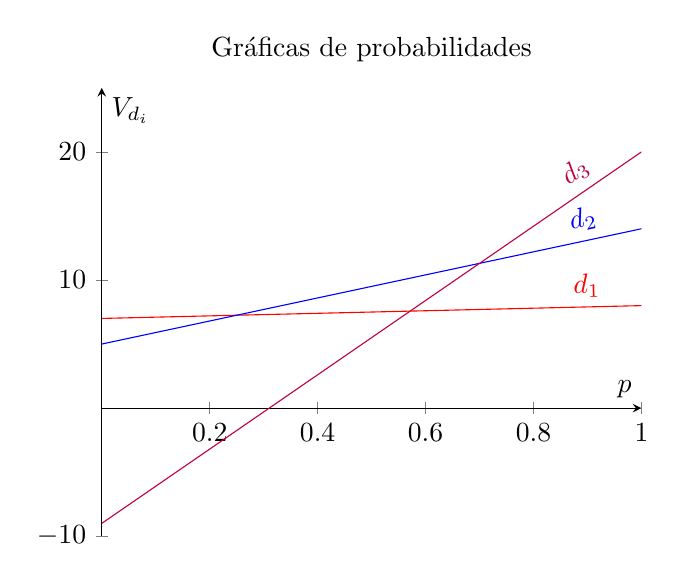
\begin{tikzpicture}
        \begin{axis}[
                xmin=0, xmax=1,
                ymin=-10, ymax=25,
                axis lines=middle,
                xlabel=$p$, ylabel=$V_{d_i}$,
                title={Gráficas de probabilidades}]
            \addplot[color=red,   domain=0:1]{x + 7} node[above, sloped,pos=0.9]{$d_1$};
            \addplot[color=blue,  domain=0:1]{9*x + 5} node[above, sloped,pos=0.9]{$d_2$};
            \addplot[color=purple, domain=0:1]{29*x - 9} node[above, sloped,pos=0.9]{$d_3$};
        \end{axis}
    \end{tikzpicture}
\end{figure}


\subsection[Rangos para el cambio de Decisión]{Determinación de Rangos para el cambio de decisión según el valor de la probabilidad "p"}
Observando el gráfico inicial, vemos dos puntos de interés: donde se encuentra el gráfico de la decisión $d_1$ con $d_2$, y $d_2$ con $d_3$.

Podemos encontrar estos puntos igualando las ecuaciones, tal que:

\insertaligned[\label{eqn:d1d2}]{
    V_{d_1} &= V_{d_2}   \\
    p + 7 &= 9p + 5      \\
    8p &= 2              \\
    p &= 0.25
}

\insertaligned[\label{eqn:d2d3}]{
    V_{d_2} &= V_{d_3}   \\
    9p + 5  &= 29p - 9   \\
    20p &= 14              \\
    p &= 0.7
}

Tenemos entonces, a partir de estos resultados y un poco de análisis del gráfico antes entregado, las siguientes situaciones:

\begin{itemize}
    \item \textit{Si $p$ está entre 0.00 y 0.25: } se debe tomar la decisión de construir un edificio \textbf{pequeño}.
    \item \textit{Si $p$ está entre 0.25 y 0.70: } se debe tomar la decisión de construir un edificio \textbf{mediano}.
    \item \textit{Si $p$ está entre 0.70 y 1.00: } se debe tomar la decisión de construir un edificio \textbf{grande}.
\end{itemize}

\pagebreak